\toggletrue{image}
\toggletrue{imagehover}
\chapterimage{existence_proof}
\chapterimagetitle{EXISTENCE PROOF}
\chapterimageurl{https://xkcd.com/1856/}
\chapterimagehover{Real analysis is way realer than I expected.}

\chapter{Einwegfunktionen}
\label{chapter-einwegfunktionen}

In diesem Kapitel werden die mathematischen Grundlagen für die Schlüsselfestlegung und asymmetrischen Kryptosysteme erklärt. Die Lernziele lauten wie folgt:


\newcommand{\einwegfunktionenLernziele}{
\protect\begin{todolist}
\item Sie erklären, was eine Funktion ist und bestimmen (falls möglich) die Umkehrfunktion.
\item Sie erklären, was eine Einwegfunktion ist und geben (mathematische) Beispiele.
\item Sie erklären das Einsatzgebiet von Einwegfunktionen.
\item Sie erklären die Idee von Einwegfunktionen mit einer Falltür.
\end{todolist}
}

\lernziel{\autoref{chapter-einwegfunktionen}, \nameref{chapter-einwegfunktionen}}{\protect\einwegfunktionenLernziele}

\einwegfunktionenLernziele

\section{Funktionen}

Eine Funktion beschreibt eine Beziehung zwischen zwei Mengen. Die Beziehung der Mengen kann man unterschiedlich darstellen. Man kann die Elemente beider Mengen zeichnen und durch Pfeile miteinander verbinden (siehe \autoref{figure-funktion-mengendarstellung}), man kann einen Funktionsgraphen zeichnen (siehe \autoref{figure-funktion-graph}) oder man kann eine Funktionsgleichung notieren ($f(x) = 2 \cdot x + 1$). Meist verwendet man eine Funktionsgleichung, da dies die kompakteste und vollständigste Darstellung ist.

\begin{figure}[htb]
	\centering
	\begin{minipage}{0.4\textwidth}
		\centering
		\begin{tikzpicture}[
    elems/.style = {
        minimum width=1.4em,
        anchor=base
    },
   	]
    \foreach[count=\i] \lseti/\lsetmi in {{A}/{-1, 2, 42, 8}, {B}/{1, 5, 85, 17}} {
        \begin{scope}[local bounding box=\lseti, x=2cm, y=0.5cm]
            \foreach[count=\j] \lj in \lsetmi {
                \node[elems] (n-\j-\lseti) at (\i, -\j) {\vphantom{5}\lj};
            }
        \end{scope}
        \node[ellipse, draw, fit=(\lseti), label={[elems, yshift=0.25em, name=\lseti]}]  {};
    }

    \foreach \i in {1,2,3, 4} {
        \draw[->] (n-\i-A) -- (n-\i-B);
    }
	\end{tikzpicture}
	\caption{Mengendarstellung.}
	\label{figure-funktion-mengendarstellung}
	\end{minipage}
	\hfill
	\begin{minipage}{0.5\textwidth}
		\centering
		\begin{tikzpicture}
  			\begin{axis}[axis lines=middle, xmin=-2, xmax=5, ymin=-2, ymax=12, xlabel=$x$, ylabel=$y$, tick label style={font=\tiny}]
  			\addplot+[no marks, blue, domain=-1:5, samples=20] {2*x+1};
  			\end{axis}
  		\end{tikzpicture}
  		\caption{Graph}
  		\label{figure-funktion-graph}
	\end{minipage}
\end{figure}

\begin{definition}[Funktion]
	Eine Funktion ist eine \textbf{Abbildung}, welche alle Elemente einer Menge $A$ auf Elemente einer anderen Menge $B$ abbildet. Die Menge $A$ wird \textbf{Definitionsmenge} genannt, die Menge $B$ wird \textbf{Zielmenge} genannt. Die Elemente aus der Definitionsmenge nennen wir \textbf{Argumente}, die Elemente der Zielmenge heissen \textbf{Funktionswerte}. Wir notieren die Funktion mit $f: A \rightarrow B$, $f(x) = \dots$ und $x in A$.
\end{definition}

Meist notiert man nur die Funktionsgleichung (z.B. $f(x) = x^2$), wenn die restlichen Angaben sowieso klar sind.

\section{Umkehrfunktionen}

Manche Funktionen erlauben es, die Abbildung umzukehren. Man sucht dann eine Funktion, welche jedem Funktionswert eindeutig ein Argument zuordnet. Wir nennen diese Funktion dann \textbf{Umkehrfunktion} und verwenden dafür die Notation $f^{-1}(x)$. 

\begin{example}
	Wir untersuchen die Funktion $f(x) = 2 \cdot x + 1$. Wir setzen für den Funktionswert die Variable $y$ ein und formen die Funktionsgleichung um: $y = 2 \cdot x + 1 \Leftrightarrow y -1 = 2 \cdot x \Leftrightarrow \frac{y-1}{2} = x$
	Wir erhalten die Umkehrfunktion $f^{-1}(y) = \frac{y-1}{2}$
\end{example}

\subsection{Aufgaben}

\begin{enumerate}
	\item Ermitteln Sie für $f(x) = 6 \cdot x - 8$ die Umkehrfunktion.
	\item Ermitteln Sie für $f(x) = log_2(x)$ die Umkehrfunktion.
	\item Ermitteln Sie für $f(x) = x^2+1$ die Umkehrfunktion.
\end{enumerate}

\section{Einwegfunktionen}

In der Kryptologie ist man an Funktionen interessiert, welche sich leicht berechnen lassen, jedoch nicht effizient umkehren lassen.

\begin{definition}[Einwegfunktion (eng. one-way function)]
	Eine Einwegfunktion ist eine Funktion $f$ mit folgenden beiden Eigenschaften:
	\begin{itemize}
		\item Die Funktion $f$ ist effizient berechenbar.
		\item Die Umkehrfunktion $f^{-1}$ ist nicht effizient berechenbar.
	\end{itemize}
\end{definition}

Man sucht also diejenigen Funktionen, für die ein Algorithmus existiert, der $f(x)$ in vernünftiger Zeit berechnen kann, aber $f^{-1}(y)$ nicht.

\begin{hinweis}
	Es ist bis heute nicht klar, ob die als Einwegfunktionen identifizierten Funktionen auch wirklich Einwegfunktionen sind. Die Menschheit hat bisher keinen Beweis dafür geliefert, dass es wirklich Einwegfunktionen sind (oder nicht). Man vermutet jedoch stark, dass es wirklich Einwegfunktionen sind. Für die Praxis gehen wir also davon aus, dass die vorgestellten Einwegfunktionen hinreichend \say{gute Einwegeigenschaften} besitzen.
\end{hinweis}

% https://computersciencewiki.org/index.php/One-way_function

\autoref{figure-one-way-function} zeigt die Idee der Einwegfunktion an einem Alltagsbeispiel.

\begin{figure}[htb]
	\centering
	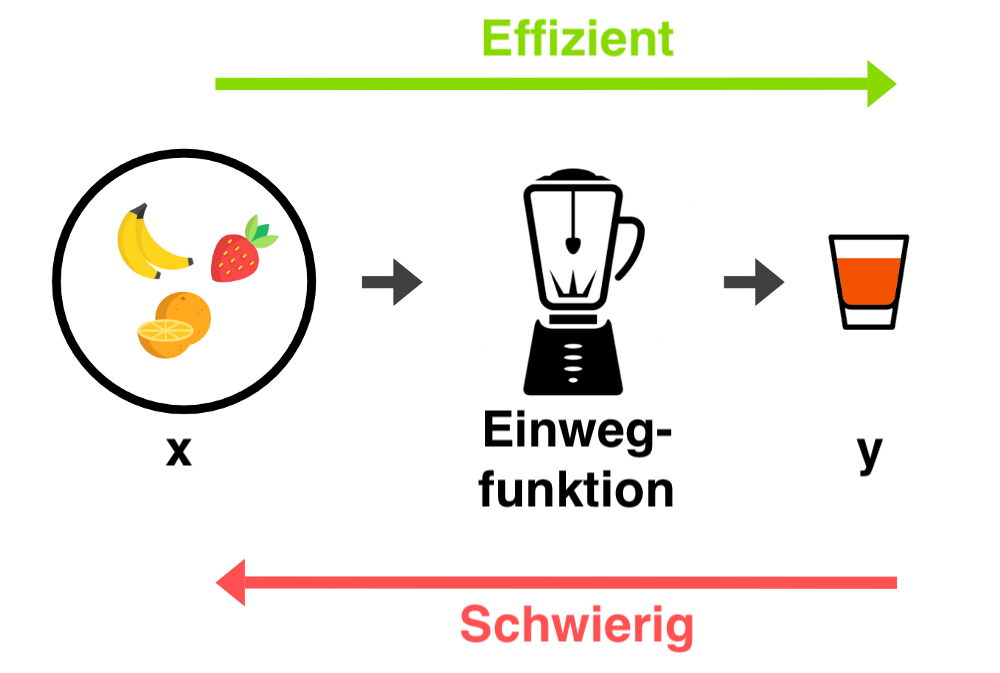
\includegraphics[scale=0.2]{one_way_function}
	\caption{Das Erstellen eines Smoothies ist effizient möglich mit einem Mixer. Die Umkehrung ist sehr schwer möglich oder sogar unmöglich.}
	\label{figure-one-way-function}
\end{figure}

\subsection{Modulares Potenzieren}

Das modulare Potenzieren ist ein Beispiel für eine Einwegfunktion. Wir betrachten dabei die Funktion $f: \mathbb{Z}_p^* \rightarrow \mathbb{Z}_p^*$ für eine Primzahl $p$. Die Funktionsgleichung lautet dann:
\begin{align*}
	f(x) = x^c \bmod p
\end{align*}
Mit einer natürlichen Zahl $c$. Dabei können wir effizient die modulare Potenz berechnen.

\begin{example}
	Wir berechnen $f(5)$ mit $c = 3$ und $p = 17$, das heisst:
	\begin{align*}
		f(5) = 5^3 \bmod 17 = 125 \bmod 17 = 6
	\end{align*}
\end{example}

Es ist aber nicht für jede Wahl von $p$ und $c$ möglich, die Umkehrfunktion in vernünftiger Zeit zu berechnen. Für die Umkehrfunktion ist ein Algorithmus notwendig, der die folgende Gleichung löst:
\begin{align*}
y = x^c \bmod p
\end{align*}

Man beachte, dass hier die Zahlen für $y$, $c$ und $p$ gegeben sind und der Wert für $x$ gesucht ist.

\begin{example}
	Für $y = 3$, $c = 2$ und $p = 11$ wird die Umkehrfunktion durch folgende Gleichung beschrieben:
\begin{align*}
3 = x^2 \bmod 11
\end{align*}
	Man muss nun den passenden Wert für $x$ ermitteln. Dies kann man für diese kleine Zahlen noch mit \say{Ausprobieren} lösen:
\begin{multicols}{2}
\begin{itemize}
		\item $1^2 \bmod 11 = 1 \bmod 11 = 1 \neq 3$
		\item $2^2 \bmod 11 = 4 \bmod 11 = 4 \neq 3$
		\item $3^2 \bmod 11 = 9 \bmod 11 = 9 \neq 3$
		\item $4^2 \bmod 11 = 16 \bmod 11 = 5 \neq 3$
		\item $5^2 \bmod 11 = 25 \bmod 11 = 3$
\end{itemize}
\end{multicols}
	Aus diesen Rechnungen kann man erkennen, dass $x = 5$ sein muss, damit die Gleichung erfüllt ist.
\end{example}

Das modulare Potenzieren stellt somit eine Einwegfunktion dar. Die Einwegfunktion wird typischerweise als \textbf{Diskretes-Logarithmus-Problem} bezeichnet.

\subsection{Aufgaben}

Finden Sie für folgende Gleichungen den passenden Wert für $x$.

\begin{enumerate}
	\item $7 = x^3 \bmod 19$
	\item $46 = x^4 \bmod 53$
	\item $56 = x^{26} \bmod 103$
\end{enumerate}

\subsection{Multiplikation zweier Primzahlen}

Die Multiplikation zweier Primzahlen stellt ebenfalls eine Einwegfunktion dar. Wir betrachten dabei die Funktion $f: \mathbb{P} \rightarrow \mathbb{P}$ mit $\mathbb{P}$ als Menge der Primzahlen. Die Funktionsgleichung lautet dann:
\begin{align*}
	f(p, q) = p \cdot q
\end{align*}
Mit $p$ und $q$ (zwei Argumente) aus der Menge $\mathbb{P}$. Dabei können wir effizient zwei Primzahlen miteinander multiplizieren.

\begin{example}
	Wir berechnen $f(7, 17)$, das heisst:
	\begin{align*}
		f(7, 17) = 7 \cdot 17 = 119
	\end{align*}
\end{example}

Es existiert aber kein effizienter Algorithmus, der die Umkehrung durchführen kann. Die Umkehrfunktion
\begin{align*}
	f^{-1}(n) = (p, q)
\end{align*}
ist nicht für jedes $n$ in vernünftiger Zeit berechenbar. Dabei muss man für eine gegebene Zahl $n$ die beiden Primzahlen herausfinden, sodass deren Multiplikation die gesuchte Zahl ergibt. Diese Berechnung nennt sich \textbf{Primfaktorzerlegung} und ist ein schwieriges Problem.

\begin{example}
	Wir sollen für $f^{-1}(3953)$ die beiden Primfaktoren $p$ und $q$ ermitteln. Man kann dies von Hand versuchen zu berechnen oder ein Online-Tool verwenden. Für kleine Zahlen ist es noch möglich und man erhält $p = 59$ und $q = 67$.
\end{example}

Die Multiplikation zusammen mit der Primfaktorzerlegung ist somit eine Einwegfunktion. Die Einwegfunktion wird typischerweise als \textbf{Faktorisierungsproblem} bezeichnet.

\subsection{Aufgaben}

Faktorisieren Sie die folgenden Zahlen in eine Multiplikation zweier Primzahlen.

\begin{enumerate}
	\item $n = 77$
	\item $n = 2911$
	\item $n = 293141$
\end{enumerate}

\subsection{Einsatzgebiet von Einwegfunktionen}

% Quelle: https://www2.informatik.hu-berlin.de/Forschung_Lehre/algorithmenII/Lehre/WS2002-2003/Perlen/Variationen.pdf

Eine Einwegfunktion kann im Allgemeinen nicht direkt zum  Verschlüsseln von beliebigen Klartexten benutzt werden. Dies liegt daran, dass der Empfänger den Kryptotext wieder entschlüsseln muss. Nutzt man eine Einwegfunktion zum Verschlüsseln, dann ist gerade dies nicht möglich. Das Entschlüsseln entspricht nämlich der Umkehrfunktion, welche bei Einwegfunktionen ja nicht effizient berechenbar ist. Trotzdem gibt es zwei populäre Einsatzgebiete:

\begin{itemize}
	\item Überprüfung der Echtheit von Nachrichten (Authentifizierung)
	\item Schlüsselvereinbarung und Schlüsselverteilung
\end{itemize}

Man kann das Konzept von Einwegfunktionen erweitern und dann damit ein Kryptosystem konstruieren. Man benötigt dazu Einwegfunktionen mit einer Falltür.

\subsection{Aufgabe}

Finden Sie drei Beispiele für eine \say{Einwegfunktion} aus dem Alltag.

% Telefonbuch: Name => Nummer ist einfach, Nummer => Name ist schwierig
% Coca-Cola: Zutaten => Cola ist einfach, Cola => Zutaten ist schwierig
% Farben: F1, F2 => Mischen ist einfach, Gemischte Farbe => F1, F2 ist schwierig
% Zahnpasta aus der Tube drücken

\section{Einwegfunktionen mit einer Falltür}

Möchte man Einwegfunktionen zur Verschlüsselung benutzen, dann muss der Empfänger in der Lage sein, die verschlüsselte Nachricht zu entschlüsseln. Dies ist mit einer gewöhnlichen Einwegfunktion nicht möglich. Es gibt jedoch Einwegfunktionen, welche die Umkehrung erlauben, sofern man eine Zusatzinformation zur Umkehrung kennt.

\begin{definition}[Einwegfunktion mit einer Falltür (eng. trapdoor one-way function)]
	Eine Einwegfunktion mit einer Falltür ist eine Funktion $f$ mit folgenden Eigenschaften:
	\begin{itemize}
		\item Die Funktion $f$ ist effizient berechenbar.
		\item Die Umkehrfunktion $f^{-1}$ ist \textbf{ohne die Falltür} nicht effizient berechenbar.
		\item Die Umkehrfunktion ist \textbf{mit der Falltür} effizient berechenbar.
	\end{itemize}
\end{definition}

Die Falltür stellt die geheime Zusatzinformation dar. Der Besitz der Falltür gibt dem Empfänger die Möglichkeit einen Kryptotext zu entschlüsseln.

\begin{important}
	Eine Einwegfunktion mit einer Falltür muss so konstruiert sein, dass man mit der Kenntnis der Falltür für ein beliebiges $y$ die Umkehrfunktion $f^{-1}(y)$ berechnen kann. Es braucht also nicht mehrere Falltüren.
\end{important}

Wir haben bisher keine konkrete Einwegfunktion mit einer Falltür gesehen. Sowohl das Diskrete-Logarithmus-Problem, als auch das Faktorisierungsproblem sind Einwegfunktionen, welche keine Falltür besitzen. Man kann sich deshalb durchaus fragen, ob es diese Art von Funktionen überhaupt gibt. Wir werden hier zunächst die Idee einer Einwegfunktion skizzieren und zeigen in einem anderen Kapitel die Existenz von Einwegfunktionen mit einer Falltür und deren Einsatz für asymmetrische Kryptosysteme. Eine Einwegfunktion mit einer Falltür kann dabei sehr vielfältig sein. Es muss keine typische arithmetische Funktion mit Rechenoperatoren sein.

\begin{example}[Einwegfunktion mit einer Falltür aus dem Alltag]
	Ein klassischer Briefkasten stellt eine Einwegfunktion mit Hintertür dar. Jeder kann einen Brief effizient einwerfen, doch das Herausholen des Briefs ist schwierig und nicht effizient machbar. Es sei denn, man besitzt den Schlüssel für den Briefkasten. Der Schlüssel für den Briefkasten stellt die Falltür dar.
\end{example}

\begin{figure}[htb]
	\centering
	\caption*{POD BAY DOORS (\url{https://xkcd.com/375/})}
	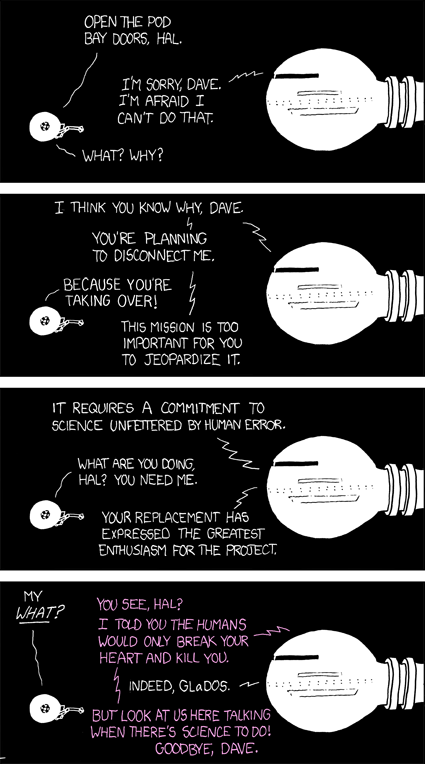
\includegraphics[scale=0.5]{pod_bay_doors}
	\caption{As they're both unplugged, they do a lovely Daisy Daisy/Still Alive duet.}
\end{figure}
